\chapter{Introduction \label{chap_1}}

\section{DNA}
DNA is the code of life. Almost all living organisms (exception: some viruses) are coded by four nucleotides: adenine (A), thymine (T), guanine (G), and cytosine (C). DNA has a double helix structure which is composed of sugar molecules, phosphate group, and bases (A, G, C, T). In DNA strands, A is always matched with T and G is always matched with C (\cite{jones2004introduction}).
DNA can copy itself through the replication process. It can also transcript into RNA. During transcription, the information in DNA pairs is passed 
to corresponding RNA, which will use uracil (U) instead of thymine (T) to match adenine. After transcription, RNA will be translated into amino acid chains then further form proteins. In the process of transcription, every three nucleotides (codon) will determine one kind of amino acid. Proteins are strings of amino acids. Figure \ref{fig_trans_trans} shows the transcription and translation process in a cell. 
\begin{figure}[!h]
\begin{center}
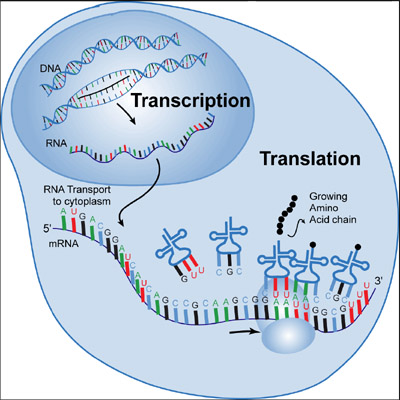
\includegraphics[height = 9cm, width = 9cm]{img/transcp_transla.jpg}
\caption[Illustration of transcription and Translation]{Illustration of transcription and Translation. DNA is transcripted to RNA. RNA is then translated to amino acid chains. From: tokresource.org\label{fig_trans_trans}}
\end{center}
\end{figure}

\section{Protein}
One or more amino acid chain forms a protein. Proteins are large biomolecules, or macromolecules. In general, proteins are made of twenty kinds of amino acids. The function of proteins varies including working as antibodies, contractile proteins, enzymes, hormonal proteins, structural, storage proteins, transport proteins, etc. (\cite{white1959principles}). Proteins are essential to organisms and participate in virtually every  process within cells. It is estimated that human body has 1 to 3 billion proteins \cite{milo2013total}.

As shown in Figure \ref{fig_pro_se}, the primary structure of a protein is its amino acid sequence. This information is the most available data we can obtain through publicly available databases such as Uniprot (\url{https://www.uniprot.org/}) \cite{uniprot2014uniprot}. For example, manually annotated all human proteins and their sequences can be downloaded by clicking on``Swiss-Prot" and then ``Human" and then ``Download". Uniprot contains additional information such as function and gene ontology information which can be filtered by editing ``Columns" before downloading. The downloaded dataset  can be further processed based on specific needs.
\begin{figure}[!ht]
\begin{center}
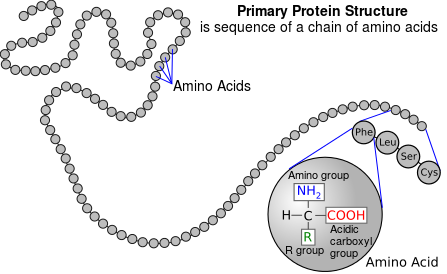
\includegraphics[ width = 8cm]{img/pro_amin.jpg}
\caption[The primary structure of a protein]{The primary structure of a protein. Each small circle indicates an amino acid, and the primary structure of a protein is the amino acid sequence. From: wikimedia.org \label{fig_pro_se}}
\end{center}
\end{figure}

As shown in Figure \ref{fig_pro_1234}, proteins also have second, tertiary, and quaternary structures. Protein secondary structure represent local structures stabilized by hydrogen bonds within a protein chain itself. The most common local structures are alpha helix and beta pleated sheet. The tertiary structure contains he overall shape of a single protein molecule, in other words, the spatial relationship of the secondary structure of multiple chains. The term "tertiary structure" is often used as interchangeably with the term "fold". The tertiary structure controls the basic function of a protein. The quaternary structure describes the structure among several protein molecules, which is a protein complex. 
\begin{figure}[!h]
\begin{center}
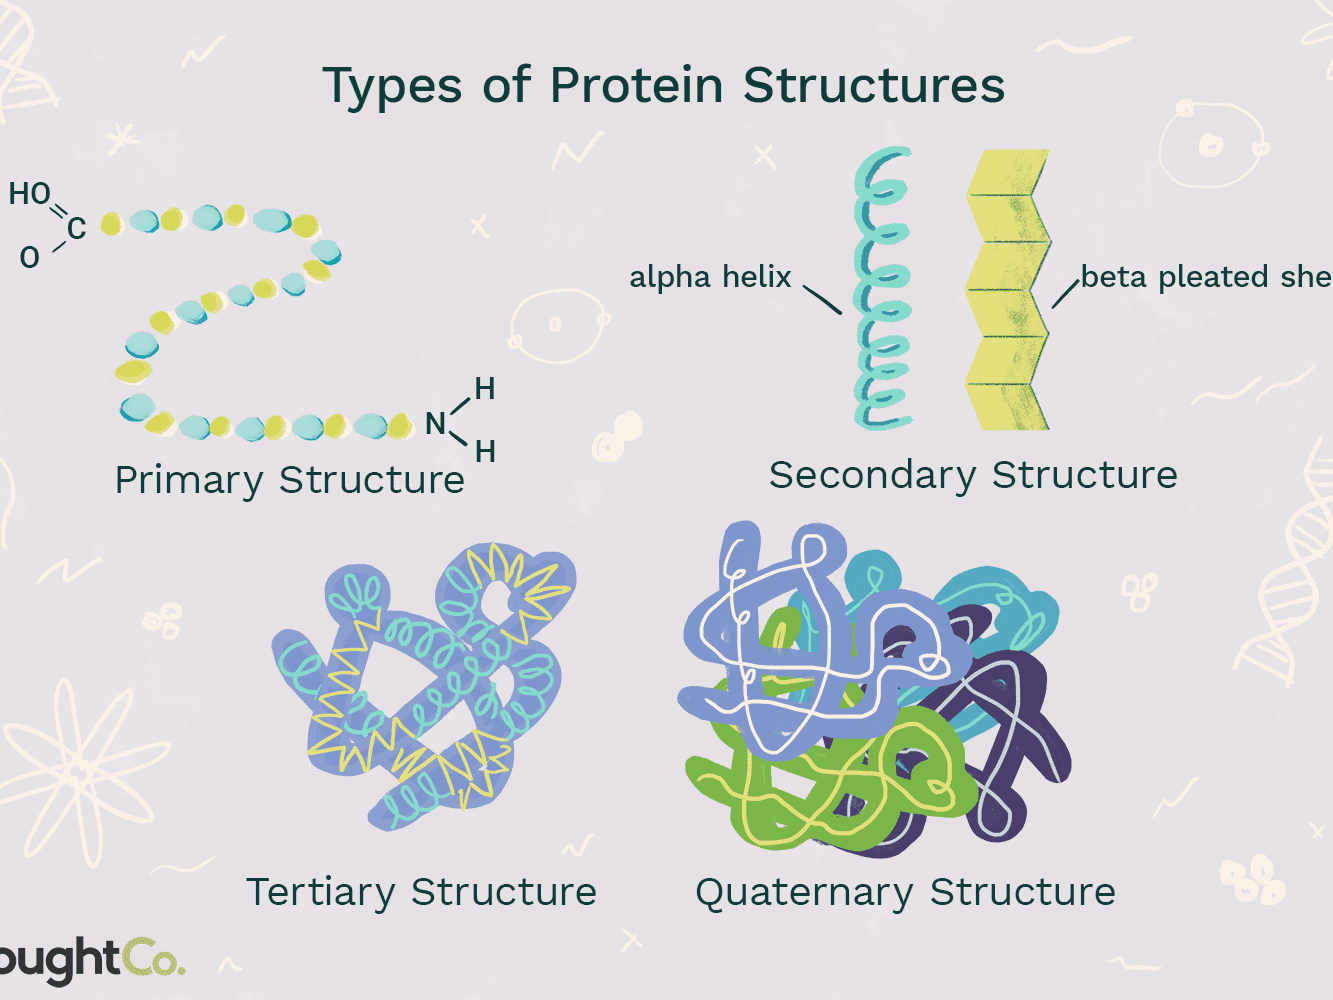
\includegraphics[ width = 12cm]{img/protein_1234_structure.png}
\caption[The primary, secondary, tertiary, and quaternary structure of proteins]{The primary, secondary, tertiary, and quaternary structure of proteins. From: https://www.thoughtco.com/ \label{fig_pro_1234}}
\end{center}
\end{figure}

As mentioned above, the most widely available data is the primary structure data of organisms. FASTA format is used to represent such data. The FASTA file uses single-letter codes to represent peptide sequences of each protein. Each protein has two lines. The first line is the protein name, and the second line is its amino acid sequence. The line containing protein names starts with a '\textgreater' sign and is followed by the protein name. In the sequence line, each letter encodes an amino acid. An example is given in Fig \ref{fig:fasta}, the amino acid sequence of protein P32479 is MKVVKFPWLAHREESRKYEIYTVDVSHDGKRLA. 

\begin{figure}
\begin{center}
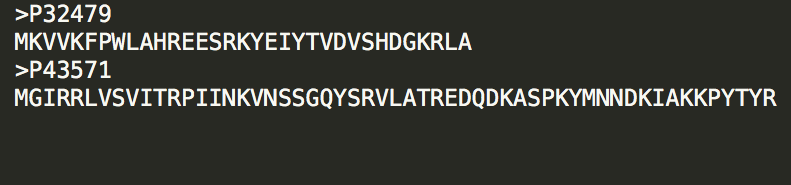
\includegraphics[width=0.8\textwidth]{img/fasta.png}
\caption[A FASTA file example]{A FASTA file example. Each protein consists of the protein name which starts with `\textgreater' and the amino acid sequence.}
\label{fig:fasta}  
\end{center}
\end{figure}

\section{Protein-protein Interaction Prediction \label{PPI_site_intro}}
Protein is the most important molecules in cells (\cite{schleif1993genetics}). 
They carry out most of the cellular processes. Quite often, they keep the cells functioning by interacting with other proteins in stable or transient protein complexes (\cite{eisenberg2000protein}).
This process is called protein-protein interaction (PPI). This is a vital process because of the accepted idea that PPIs are responsible for the behaviour of cells under different stimuli (\cite{bader2003functional, pandey2000proteomics, schwikowski2000network}).
Protein complexes are groups of proteins that interact together to perform certain functions. Figure \ref{fig_pro_comp} shows an example of a protein complex. Protein pathways and modules are another two functional groups connected through PPIs. 
\begin{figure}[h!]
\begin{center}
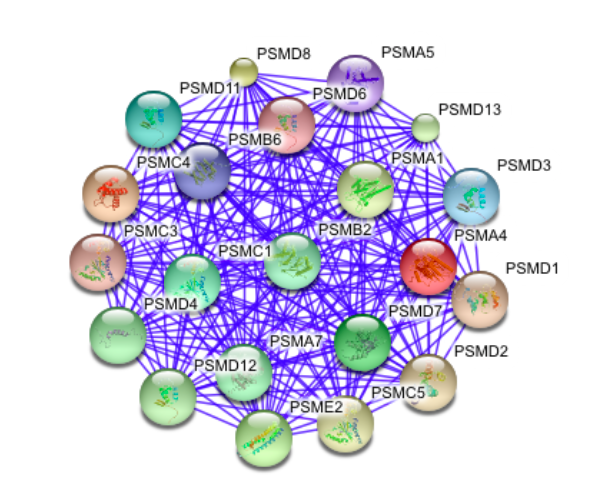
\includegraphics[height = 8cm]{img/pro_comp.png}
\caption[Protein complex]{Protein complex. (From: bioproximity.com)  \label{fig_pro_comp}}
\end{center}
\end{figure}
 Scientists believe the reason that advanced organisms like humans are more complicated than lower organisms like the worms is not only because of large number of genes, but also because of sophisticated PPI networks \cite{pitre2008computational}. Figure \ref{fig_ppi_net} shows a illustration of human PPIs.
Understanding the potential of unknown proteins is becoming possible by looking into their PPI information \cite{sharan2007network}. As well, ientifying PPI information helps improve the system-level understanding of molecular processes \cite{levy2008evolution}.
Therefore, understanding and mapping PPIs is an important current area of research.

\begin{figure}[h!]
\begin{center}
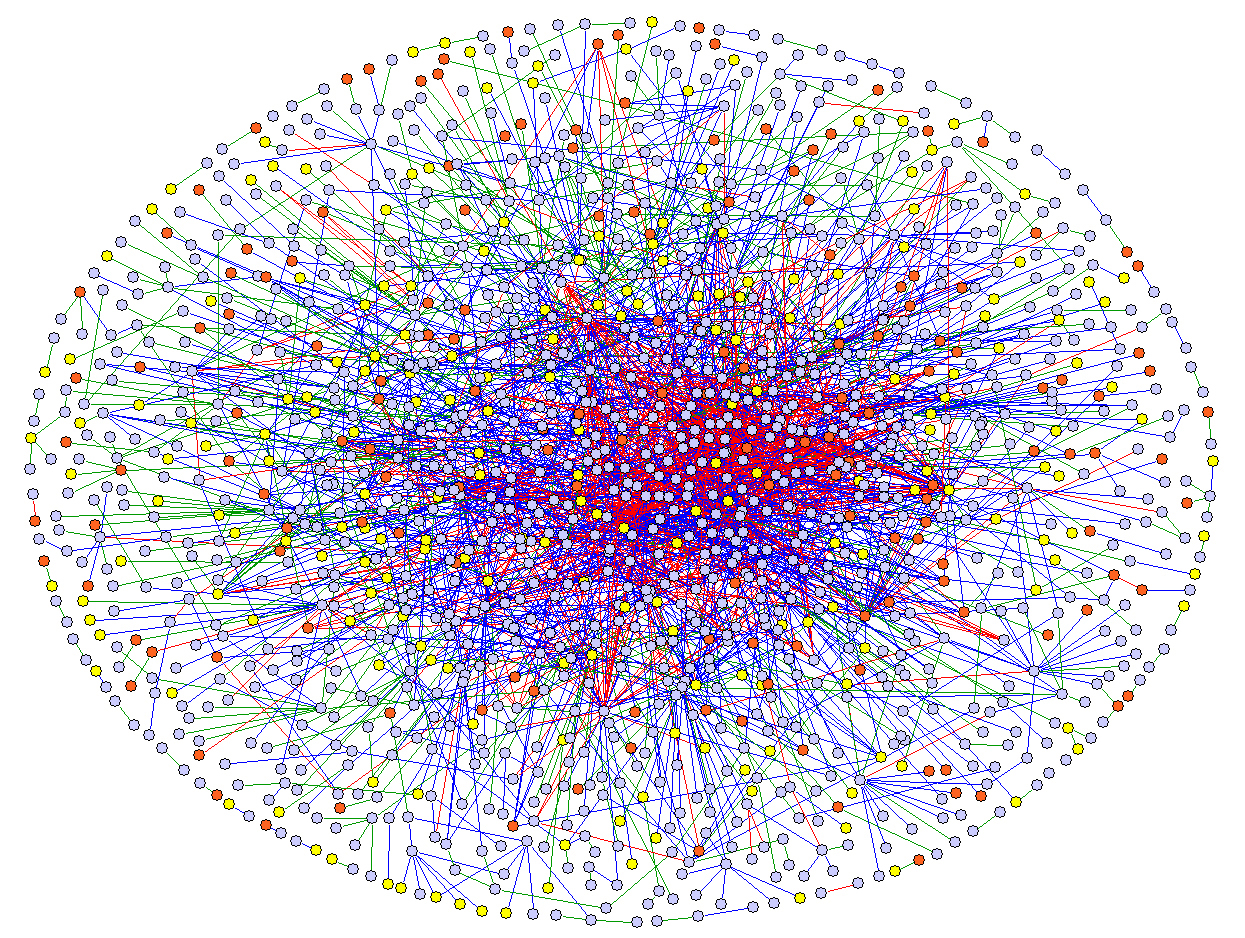
\includegraphics[height = 10cm, width = 10cm]{img/pro_inter_net.jpg}
\caption[A human protein-protein interaction network]{A human protein-protein interaction network. (From: \href{https://www.mdc-berlin.de/}{www.mdc-berlin.de})  \label{fig_ppi_net}}
\end{center}
\end{figure}

However, there are a lot of unknown facts about PPIs to be discovered. For example, in a simple organism such as Saccharomyces Cerevisiae, there are less than 40,000 estimated PPIs. Comparing with 19,000,000 potential interacting pair, it is believed that there is still a significant gap between discovered PPIs and all PPIs of existence \cite{jessulat2011recent, sprinzak2003reliable}. Precise, fast and affordable protein-protein interaction prediction methods are needed.

The idea of PPI prediction is shown in Figure \ref{fig_ppi_pred}. Proteins and interactions are indicated using nodes and edges respectively. Green edges are known interactions. Red edges are unknown interactions. The task of predicting PPIs is to add the red edges. 
\begin{figure}[h!]
\begin{center}
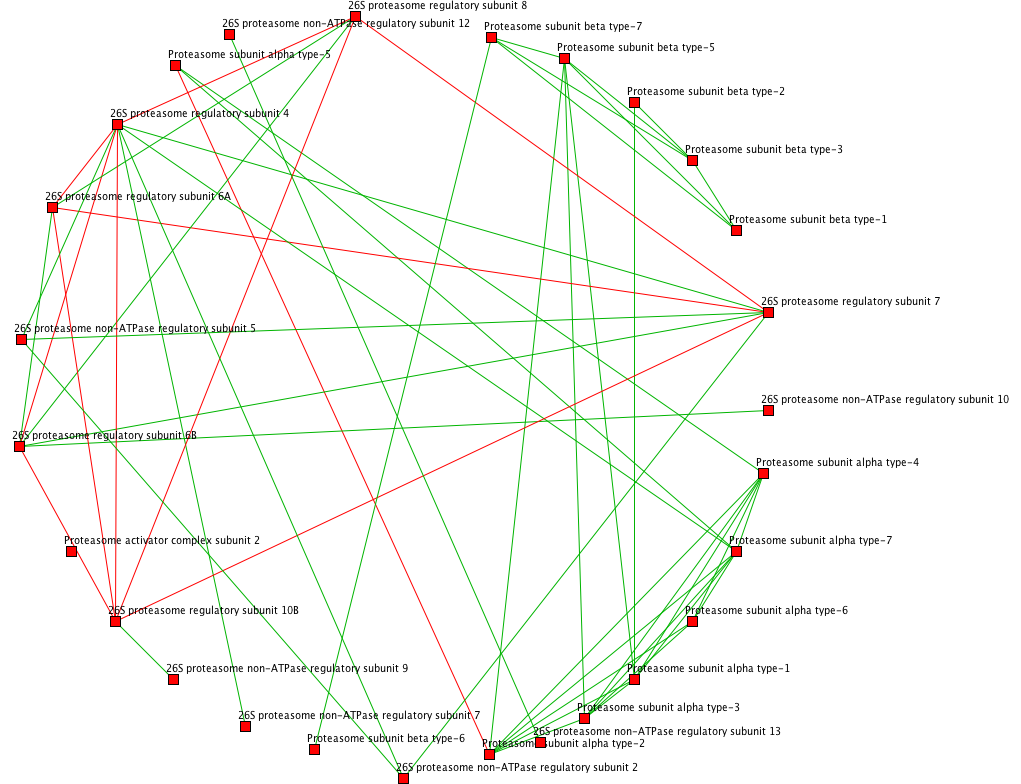
\includegraphics[width=12cm]{img/network.png}
\end{center}
\caption[The idea of protein-protein interaction prediction]{The idea of protein-protein interaction prediction. The red dots indicate proteins and edges mean interactions. Green edges are discovered interactions stored in PPI databases. The idea of predicting PPIs is to add the red edges, which indicate interactions that exist but are missing in the database. \label{fig_ppi_pred}}
\end{figure}

In additional to the protein primary sequences, stored in FASTA file (see Figure \ref{fig:fasta}), protein-protein interaction file is also needed for PPI prediction (see Figure \ref{fig_ppi_input_output} left). PPI files contain known interactions from databases that help PPI predictors learn to classify new interactions, together with the sequence information. Most machine learning based programs also require as an additional input, the negative interactions, that is protein pairs that are known not to interact. The output of PPI predictors are scores for each new protein pair (see Figure \ref{fig_ppi_input_output} right). The higher the score, the more confident a predictor claims a pair of proteins interact.
\begin{figure}[h!]
\begin{center}
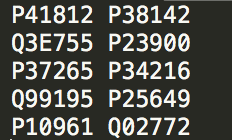
\includegraphics[width=7cm]{img/ppi_file.png}
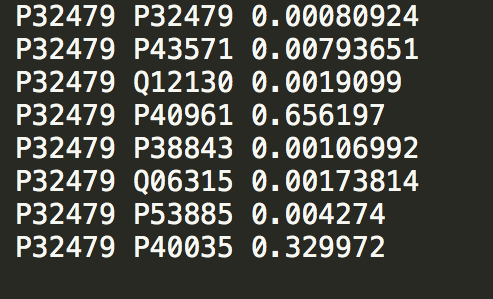
\includegraphics[width=7cm]{img/result_interactome.png}
\end{center}
\caption[Examples of an input PPI file and output PPI score file]{Examples of an input PPI file (left) and output PPI score file (right). \label{fig_ppi_input_output}}
\end{figure}

\section{Protein-protein Interaction Binding Sites Prediction}
Proteins interact with each other by binding together. Figure \ref{fig_ppi_bind} shows two binding proteins. The bonding amino acid residues are protein-protein interaction binding sites. Detecting PPI binding sites helps understand cell regulatory mechanisms, locating drug target, predicting protein functions \cite{bonetta2010interactome}. There are noticeable industrial efforts putting into this area as well. For example, RemediumAI (remediumai.com) is developing machine learning predictors to accelerate the drug design process. Databases like PDB \cite{berman2002protein} store protein binding sites information deriving from the 3D structure of each protein, but the available protein structures are limited. Predicting the binding residues in each protein have been attempted by many researcher. However, the prediction performance is still far from satisfaction. 
\begin{figure}[h!]
\begin{center}
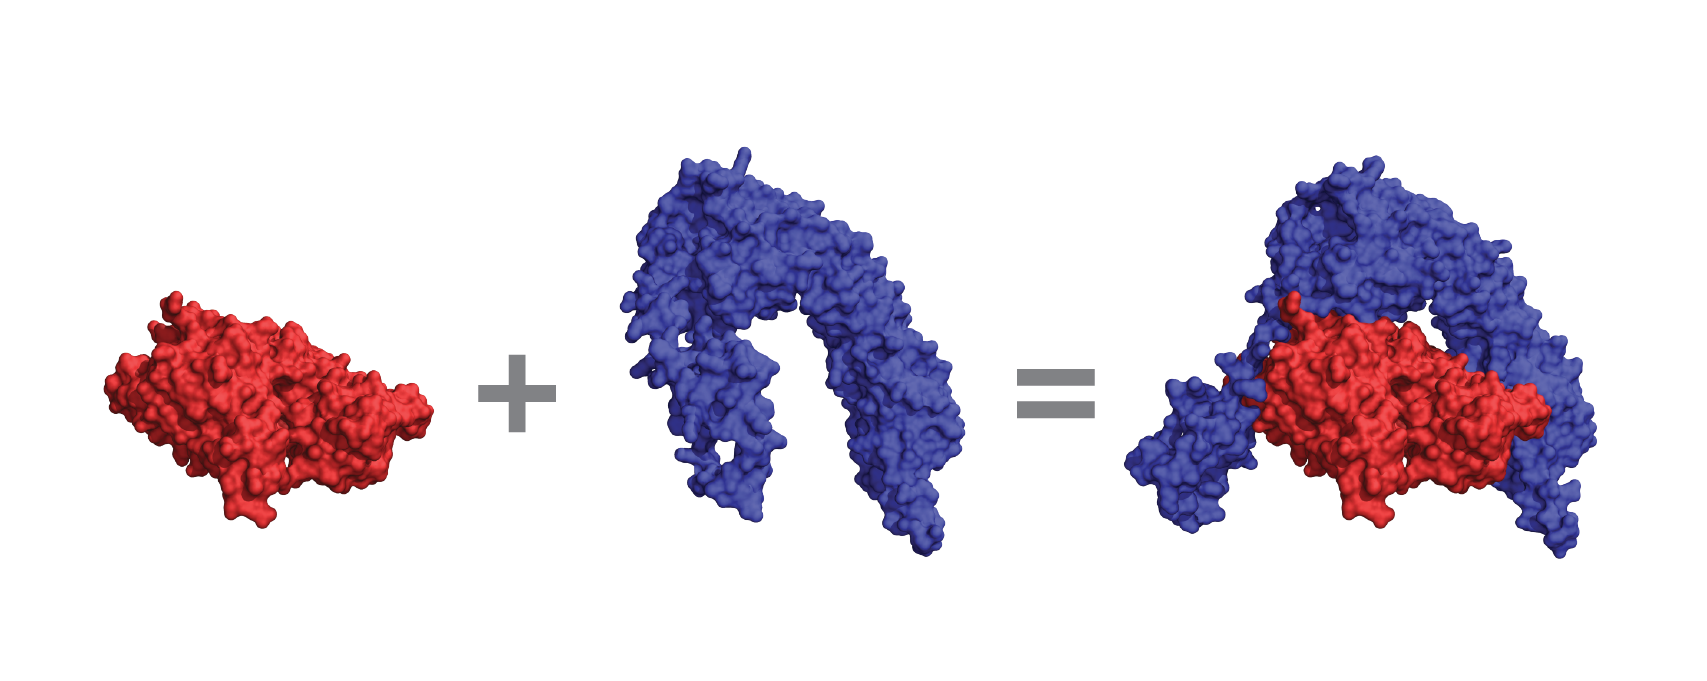
\includegraphics[width=12cm]{img/binding_sites.png}
\end{center}
\caption[Illustration of protein-protein interaction binding sites]{Protein-protein interaction binding sites. Two interaction proteins (red and blue) forms a binding structure (rightmost). The contacting residues are binding sites. (From: \cite{townshend2018generalizable}) \label{fig_ppi_bind}}
\end{figure}

Similar to the PPI prediction problem, in the realm of PPI binding sites prediction, experimental approaches, for instance, mutagenesis, are labor and time consuming, and thus, many computational PPI sites prediction programs have been developed as they are faster and cheaper. Again, there are mainly two categories: sequence based and structure based methods \cite{esmaielbeiki2016progress}. For the same reason disccussed in Section \ref{PPI_site_intro}, we focus on sequence based methods.

The illustration of PPI biding site prediction is shown in Figure \ref{fig_ppi_bind_work_flow}. Programs are trained using the primary sequence and discovered binding sites and then predict binding residues on new proteins.
\begin{figure}[h!]
\begin{center}
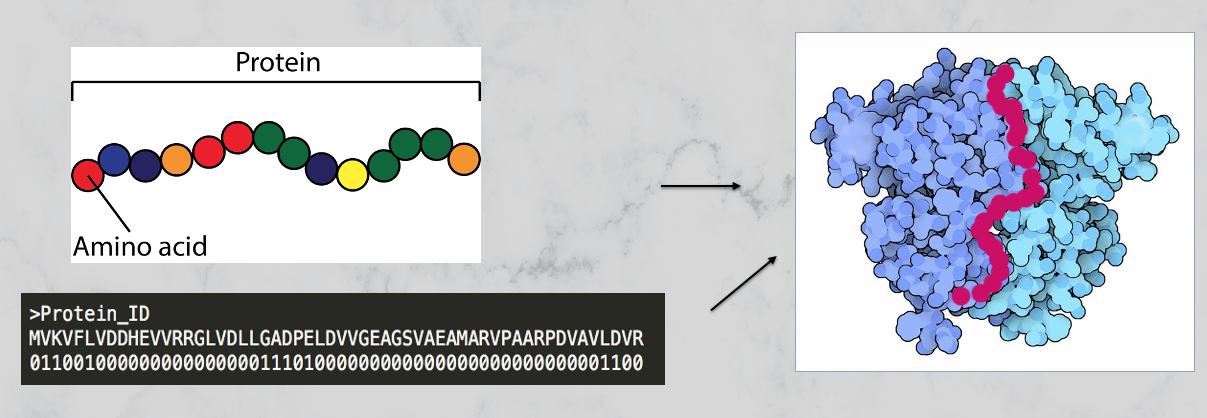
\includegraphics[width = 15cm]{img/PPI_site_pred_input.png}
\end{center}
\caption[Illustration of protein-protein interaction binding sites prediction]{Illustration of the input and output in the protein-protein interaction binding sites prediction task. On the left, the primary sequence and the biding site information are used as inputs. They are stored in a FASTA-like format where an additional line is added for each protein. 1 indicates binding sites and 0 means non-binding sites for the corresponding location. The binding sites for new proteins are predicted (red circles on the right). \label{fig_ppi_bind_work_flow}}
\end{figure}

\section{Thesis Overview}
The thesis is organized as follows. Chapter \ref{chap_1} describes the DNA, protein, and defines the problems. Chapter \ref{chap_2} describes in details our PPI sites prediction program, DELPHI \cite{li2020delphi}. Chapter \ref{chap_3} describes in details our PPI prediction program, SPRINT \cite{li2017sprint, li2020predicting}. Chapter \ref{chap_4} concludes our research contribution, summarizes some common methodologies in working in bioinformatics, proposes some future work.
